\chapter{Objectif}

L'objectif de ce rapport est de documenter le processus de développement de notre projet de jeu de plateau dans le cadre de la SAE-IHM \footnote{Voir glossaire :\hyperref[sae-ihm]{SAE-IHM}}, en mettant l'accent sur les méthodes et les étapes suivies, ainsi que sur les défis rencontrés et les solutions apportées, sans entrer dans les détails techniques du code.

\chapter{Structure et Contenu}

\section{Introduction Générale}

La création d’un jeu vidéo inspiré d’un jeu de société est un exercice complet permettant d’aborder de nombreuses problèmatique que peut rencontrer un développeur dans sa vie professionnelle.

Or, la SAE IHM (Situation d'Apprentissage et d'Évaluation en Interface Homme-Machine) vise à simuler un environnement de développement professionnel en demandant de travailler en équipe pour développer une application complète.
Un projet qui permet non seulement de renforcer des compétences techniques, mais aussi de développer des compétences en communication, en gestion de projet et en travail d'équipe. \\

Notre équipe est composé des personnes suivantes :
\begin{itemize}
    \item Tim \textsc{Carrara}
    \item Mathis \textsc{Courvoisier}
    \item Florian \textsc{Hegele}
    \item Yahia \textsc{Kherza}
    \item Olivier \textsc{Maraval}\\
\end{itemize}

Dans le cadre de cette SAE, notre équipe a choisi de développer un jeu de plateau intitulé "\textsc{Le Roi des Roses}".
Un choix motivé par la richesse stratégique du jeu et les défis techniques qu'il présente.
Nous avons été attirés par la complexité des règles et des interactions possibles, ce qui nous a offert une opportunité unique d'explorer des concepts variés en programmation et en intelligence artificielle.
Il s’agit aussi du jeu avec lequel nous avons nous même pris le plus plaisir à jouer parmis ceux proposés.\\

Le présent rapport détaille notre démarche de développement, les défis rencontrés, et les solutions apportées. Il se structure comme suit :
\begin{itemize}
    \item une présentation du jeu et de ses règles,
    \item une description de l'implémentation et des choix techniques,
    \item une analyse de l'organisation du travail,
    \item un bilan de la réalisation technique et des compétences acquises,
    \item et enfin une conclusion sur les perspectives d'amélioration.
\end{itemize}

\section{Présentation du Jeu}

Le \textsc{Roi des Roses} est un jeu de plateau stratégique se jouant à deux joueurs.
Le plateau est constitué d'une grille de 9x9 cases, avec un pion central nommé "\emph{roi}".
Chaque joueur dispose de 26 pions bifaces, rouges d'un côté et bleus de l'autre, ainsi que de 4 cartes "\emph{Héros}" et de 5 cartes "\emph{Déplacement}" tirées d'une pioche de 24 cartes.

Le but du jeu est de contrôler le plus de zones adjacentes de pions de sa couleur en déplaçant le roi sur le plateau selon les directions et distances indiquées par les cartes "\emph{Déplacement}".
Les cartes "\emph{Héros}" permettent de retourner les pions adverses, ajoutant une couche de stratégie supplémentaire.
Le jeu se termine lorsqu'aucun des deux joueur ne peut plus jouer de cartes "\emph{Déplacement}" ou lorsque tous les pions ont été placés.
Le gagnant est celui qui contrôle le plus de zones adjacentes de pions de sa couleur, avec des points calculés en fonction du nombre de pions dans chaque zone.
En cas d’égalité, le gagnant est celui qui a posé le plus de pions.

\section{Implémentation et Challenges}

\subsection{Contraintes techniques}
Le développement du jeu \textsc{Roi des Roses} a été encadré par plusieurs contraintes techniques imposées par le cadre de la SAE IHM :
\subsubsection*{Paradigme MVC (Modèle-Vue-Contrôleur) :}
Le jeu devait être développé en respectant strictement ce paradigme pour assurer une séparation claire entre la logique de l'application, l'affichage, et les interactions utilisateur.
\begin{itemize}
	\item \textbf{Modèle (Model) :} Gère les données de l'application et la logique métier.
	\item \textbf{Vue (View) :} Gère l'affichage des données et l'interface utilisateur.
	\item \textbf{Contrôleur (Controller) :} Gère les interactions de l'utilisateur, envoie les commandes au modèle pour modifier l'état des données, et met à jour la vue.
\end{itemize}
\subsubsection*{Deux versions du jeu :} 
Une version en mode texte utilisant le framework boardifier-console, et une version graphique utilisant JavaFX et le framework boardifier. La version en mode texte permet de tester la logique du jeu sans interface graphique, tandis que la version graphique offre une expérience utilisateur plus riche et interactive. Elle constitue le produit final qui serait demandé par un client.
\begin{itemize}
	\item \textbf{Version en mode texte :} Utilise le framework boardifier-console pour afficher le jeu sous forme de texte dans un terminal. Cela signifie que toutes les interactions et les affichages se font par des lignes de texte.
	\item \textbf{Version graphique :} Utilise JavaFX et le framework boardifier pour créer une interface utilisateur graphique où les joueurs peuvent interagir avec des éléments visuels comme des boutons et des images.
\end{itemize}
\subsubsection*{Langage de programmation :} 
Le jeu devait être développé en Java, avec une version conseillée de Java 17. Il s’agit d’une version LTS (Long Time Support) permettant de s’assurer que le développement ne sera pas impacté par une mise à jour du langage tout en profitant des fonctionnalités modernes et des améliorations de performance apportés par une version récente de Java.
\subsubsection*{Environnement de développement :} 
L'utilisation de l'IDE IntelliJ IDEA était requise. Il s’agit d’un logiciel qui fournit des outils complets pour écrire, tester et déboguer leur code. Une contrainte qui permet de s’assurer que toute l’équipe travaillera en utilisant un environnement similaire.
\subsubsection*{Dépôt de code :} 
Le code source devait être déposé sur le GitLab du département. GitLab est une plateforme de gestion de code source qui utilise Git, un système de contrôle de version. Cela permet de suivre les modifications apportées au code par chaque membre de l'équipe.

\subsection{Choix d'implémentation}

Pour transposer le jeu en une application, plusieurs choix ont été faits concernant l'interaction utilisateur et l'affichage :

\subsubsection*{Interface utilisateur :}
Pour jouer au jeu, l'utilisateur interagit principalement avec des cartes et des pions sur le plateau. Voici comment cela se passe dans les deux versions :
\begin{itemize}
	\item \textbf{Version texte :}
		\begin{enumerate}
			\item L'utilisateur saisit des commandes textuelles pour déplacer le roi ou jouer des cartes.
			\item Les informations sur l'état du jeu sont affichées sous forme de texte dans la console.
		\end{enumerate}
	\item \textbf{Version graphique :}
		\begin{enumerate}
			\item L'utilisateur clique sur les cartes et les pions pour effectuer des actions.
			\item Les mouvements et les actions sont animés, offrant une meilleure compréhension visuelle de l'état du jeu.
		\end{enumerate}
\end{itemize}

\subsubsection*{Phases du Jeu :}
Voici comment fonctionne la boucle principale du jeu :
\begin{itemize}
	\item \textbf{Début du jeu :}
	\begin{enumerate}
		\item Les joueurs tirent leurs cartes de déplacement et de héros.
		\item Le roi est placé au centre du plateau.
	\end{enumerate}
	\item \textbf{Tour de jeu :}
	\begin{enumerate}
		\item Le joueur actif sélectionne une carte de déplacement et déplace le roi.
		\item Si nécessaire, le joueur peut jouer une carte héros pour retourner un pion adverse.
		\item Le tour passe à l'autre joueur.
	\end{enumerate}
		\item \textbf{Fin du jeu :}
	\begin{enumerate}
		\item Le jeu se termine lorsqu'un joueur ne peut plus jouer de cartes de déplacement ou lorsque tous les pions ont été placés.
		\item Les points sont calculés en fonction des zones contrôlées par chaque joueur.
	\end{enumerate}
\end{itemize}


\subsubsection*{Animation des cartes :}
Les cartes "Déplacement" sont affichées avec leur face visible pour le joueur, et tournées en fonction de la position du roi sur le plateau. Les cartes jouées sont placées dans une fosse pour être re-mélangées et re-distribuées, sans duplication.

\subsubsection*{Interaction des pions :}
Les pions peuvent être retournés en utilisant des cartes "Héros". Cette action est animée pour montrer visuellement le changement de couleur des pions.

\subsubsection*{Intelligence Artificielle :}
Les IA dans "Roi des Roses" sont conçues pour simuler des adversaires humains en utilisant différentes stratégies. Bien que les IA actuelles ne voient pas dans le futur, elles évitent ou engagent des situations avantageuses/désavantageuses. Voici un aperçu des différentes IA implémentées :\\

\begin{itemize}
	\item \textbf{Random (Aléatoire) :}
		\subitem \textbf{\emph{Stratégie :}} Cette IA choisit ses actions de manière totalement aléatoire. Elle ne suit aucune logique spécifique, ce qui la rend imprévisible.
		\subitem \textbf{\emph{Utilisation :}} Utile pour tester la robustesse des autres IA. Peut parfois fournir un défi intéressant.\\
    \item \textbf{Camarade (Amicale) :}
        \subitem \textbf{\emph{Stratégie\footnote{Voir \hyperref[fig:cam1]{Figure C.1}} :}} Priorise la mise en place de nouveaux pions sur le plateau sans nuire directement à l'adversaire. L'objectif principal est d'étendre sa propre influence sur le plateau.
		\subitem \textbf{\emph{Utilisation :}} Simule un joueur qui cherche à maximiser sa présence sans agressivité directe. Permet des parties agréables pour apprendre le jeu sans frustration.
		\subitem \textbf{\emph{Implémentation :}} L'IA Camarade trie les actions possibles de déplacement par ordre de points décroissants et choisit la meilleure. Si aucune action de déplacement n'est possible, elle prend une nouvelle carte. En dernier recours, elle joue une carte héros.\\
        
	\item \textbf{Hate Cards (Déteste les cartes) :}
        \subitem \textbf{\emph{Stratégie\footnote{Voir \hyperref[fig:hate1]{Figure C.2}} :}} Cette IA évite de prendre de nouvelles cartes autant que possible. Elle préfère jouer les cartes de mouvement qu'elle possède plutôt que d'en tirer de nouvelles.
		\subitem \textbf{\emph{Utilisation :}} Représente un joueur qui préfère agir rapidement avec les ressources disponibles plutôt que d'accumuler des cartes.
		\subitem \textbf{\emph{Implémentation :}} L'IA Hate Cards priorise les actions de déplacement. Si aucune action de déplacement n'est possible, elle joue une carte héros. Si aucune de ces actions n'est possible, elle prend une nouvelle carte.\\
	\item \textbf{Guide (Aggressif) :}
		\subitem \textbf{\emph{Stratégie\footnote{Voir \hyperref[fig:guide1]{Figure C.3}} :}} Priorise la coupure des lignes de pions de l'adversaire. Cette IA cherche à perturber les stratégies de l'adversaire en bloquant ses mouvements.
		\subitem \textbf{\emph{Utilisation :}} Simule un joueur stratégique et agressif qui cherche à déstabiliser l'adversaire.
		\subitem \textbf{\emph{Implémentation :}} L'IA Guide priorise les actions de jeu de cartes héros en cherchant celles qui ont un impact significatif (au-dessus d'un certain seuil de pions). Si aucune action de ce type n'est possible, elle joue une carte de mouvement. En dernier recours, elle prend une nouvelle carte.
\end{itemize}


\subsubsection*{Son :}
Bien que le son ne soit pas nécessaire à l’usage du programme par l’utilisateur, ce dernier est un ajout appréciable pour le confort de jeu. Un coup joué donne un feedback auditif et une musique de fond permet d’ancrer l’ambiance du jeu dans l’imaginaire du joueur.

\section{Organisation du travail}

\subsection{Vue Globale}

\begin{figure}[!h]
    \begin{tabularx}{\textwidth}{|X|c|c|X|}
        \hline
        \textbf{Phase} & \textbf{Planifié} & \textbf{Réel} & \textbf{Commentaires} \\
        \hline
        Analyse des besoins & 1er mai - 5 mai & 1er mai - 5 mai & \\
        \hline
        Conception & 6 mai - 8 mai & 6 mai - 12 mai & Retards dus à la découverte de "boardifier" \\
        \hline
        Implémentation & 9 mai - 19 mai & 13 mai - 23 mai & Retards dus au manque de documentation "boardifier" \\
        \hline
        Tests et intégration & 9 mai - 19 mai & 13 mai - 21 mai  & Avons fini plus tôt pour nous occuper du rapport \\
        \hline
        Rapport (EN) et démonstration & 20 mai - 24 mai & 22 mai - 24 mai & Avons sur-évaluer le temps nécessaire \\
        \hline
        \textbf{Jalon 1} & 24 mai & 24 mai & \\
        \hline
        Définition du sujet & 25 mai - 25 mai & 25 mai - 26 mai & \\
        \hline
        Recherche et analyse & 26 mai - 26 mai & 27 mai - 28 mai  & \\
        \hline
        Préparation de la présentation & 27 mai - 27 mai & 29 mai - 30 mai &  \\
        \hline
        Répétition et finalisation & 28 mai - 28 mai & 31 mai - 31 mai  & \\
        \hline
        \textbf{Jalon 2} & fin mai & 31 mai  & Aucun retard, aurions pu avancer sur la version graphique \\
        \hline
        Conception graphique & 29 mai - 2 Juin & 1 Juin - 2 Juin & Peu de préparation car rendu proche \\
        \hline
        Implémentation graphique & 3 juin - 13 juin & 3 juin - 15 juin  & Retards dus à la découverte de "boardifier javafx" \\
        \hline
        Tests et intégration & 3 juin - 13 juin & 3 juin - 13 juin  & \\
        \hline
        Préparation de la soutenance & 14 juin - 15 juin & 14 juin - 15 juin  & \\
        \hline
        Rapport (FR) & 16 juin - 17 juin & 16 juin - 17 juin & \\
        \hline
        \textbf{Jalon 3} & 17 juin & 17 juin &\\
        \hline
    \end{tabularx}
    \caption{Tableau de Planification et Réalisation}
\end{figure}

\begin{figure}[h]
    \centering
    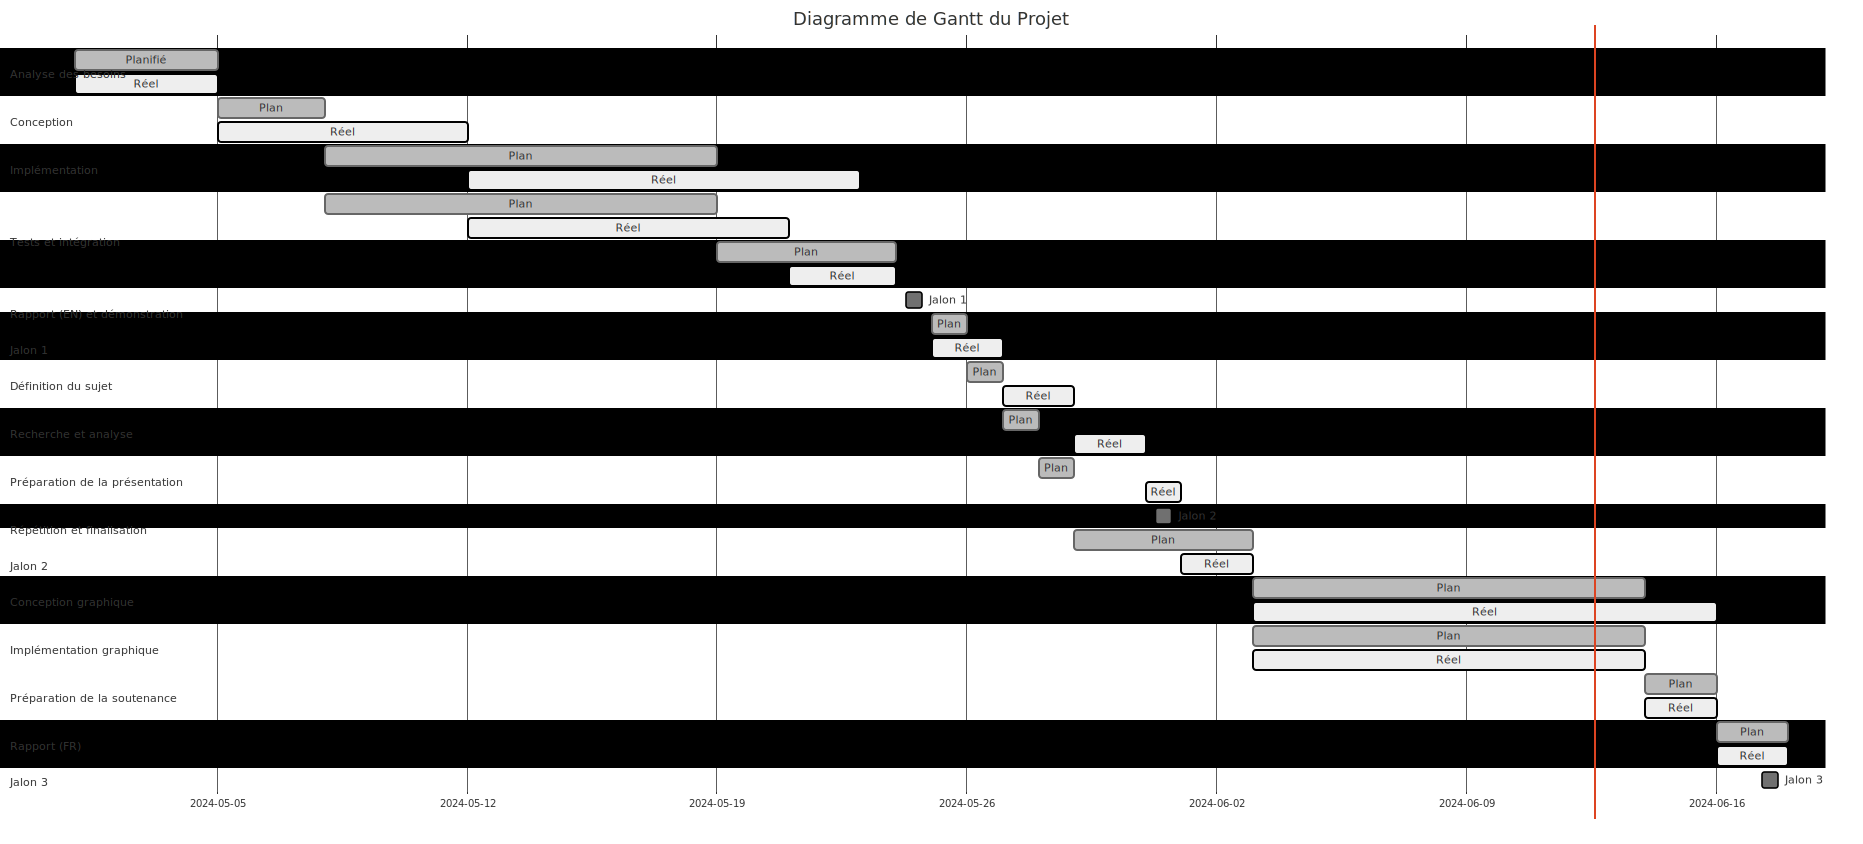
\includegraphics[width=\textwidth,angle=0]{./images/mermaid-diagram}
    \caption{Diagramme de Gantt du Projet}
    \label{fig:gantt}
\end{figure}

\subsection{Commentaires quant à l'organisation de l'équipe}

\subsubsection{Jusqu'au Jalon 1}

La SAÉ nous a été présentée en janvier, et nous avons reçu les instructions nécessaires à son commencement courant mars.
Cependant, nous avons décidé de débuter le projet début mai.
Ce choix a été motivé par la nécessité de travailler en parallèle sur une autre SAÉ, et nous avons préféré ne pas nous disperser.
Nous avons effectivement commencé le travail aux alentours du 1er mai.
Nous avions décidé que toute l'équipe travaillerait d'abord à la compréhension du framework et à la mise en place d'un document constituant le plan initial de développement de notre application.
Par la suite, l'équipe devait se diviser en deux : une partie s'occupant des tests et l'autre du développement de l'application proprement dite.

Malheuresement, peu de choses se sont déroulées comme prévu.
Bien que tout le monde ait suivi le tutoriel "The Hole", nous n'avons conçu ni maquette ni document pouvant nous guider dans la direction à prendre pour le projet.
Nous avons également rencontré un problème de compréhension lors de l'implémentation de notre jeu.
Nous n'avions pas une vision d'ensemble claire sur l'utilisation du boardifier, et avons dû produire un diagramme UML pour nous repérer plus facilement(\hyperref[fig:uml]{Voir Figure C.4}).

Lorsqu'est venu le moment d'implémenter le programme, nous nous sommes souvent bloqués, ne sachant comment travailler sans empiéter sur le travail d'un autre.
Cela a donné un mode de travail où nous étions plusieurs à réfléchir sur le même code avant de tous passer sur les tests, qui auraient dû être implémentés en parallèle du code.
Nous avons tout de même finalement réussi à nous séparer sur différentes fonctions à implémenter, mais sans trop savoir précisément qui travaillait sur quoi.

\subsubsection{Du Jalon 1 au Jalon 2}

Nous avons décidé de mettre un membre de l'équipe à temps plein sur la question de droit tandis que les autres continueraient à travailler sur l'implémentation console dans le but d'avoir un code propre et fonctionnel pour l'implémentation graphique.

\subsubsection{Du Jalon 2 au Jalon 3}

Dès la réception du nouveau framework boardifier, nous avons décidé d'une nouvelle façon de fonctionner.
Nous avons travaillé ensemble pour obtenir un premier affichage avec la nouvelle interface graphique avant de nous répartir le travail.
Une fois cette étape réalisée, nous nous sommes répartis chacune des fonctions à implémenter (menu de configuration, implémentation des IA, son, etc.) et avons développé chacun de notre côté sur une branche différente du git.

Cela s'est avéré être une façon bien plus efficace de travailler, qui nous a permis de suivre un fil d'Ariane vital à l'accomplissement de la tâche finale de cette SAÉ pour laquelle nous avions assez peu de temps.


\chapter{Bilan}

\section{Réalisation Technique}

\subsection*{Mode Texte}

Nous avons réussi à implémenter toutes les règles de base du jeu "\textsc{Roi des Roses}". Le jeu est jouable en mode texte et en mode graphique. Toutes les fonctionnalités principales, telles que le déplacement du roi, le retournement des pions avec les cartes "Héros", et la gestion des cartes "Déplacement", sont opérationnelles en mode texte et aucun bug ne nous est apparu.

Nous n'avons pas eu le temps de développer des IA complexes. Des améliorations sont nécessaires pour rendre les IA plus robustes et stratégiques comme leurs permettre de voir plusieurs coups en avance ou mettre en place un système d'apprentissage non supervisé.

Les tests ont été implémentés une fois le développement de l'application en mode console terminé. Bien qu'ils nous ai aidés à trouver certains bugs, il aurait été plus utiles de les coder en avance pour nous assurer que nos implémentations étaient fonctionnelles de manière plus efficace qu'en lançant le jeu pour vérifier.

\subsection*{Mode Graphique}

\section{Connaissances et Compétences}

\section{Etude de cas juridique}

La question "Auteur de jeu : auteur d'une œuvre ?" invite à une réflexion sur la nature de l'auteur et de l'œuvre dans le contexte des jeux. Pour y répondre, il faut définir les notions d'auteur, d'œuvre et de jeu au sens juridique.

En droit civil, l'auteur désigne la personne à l'origine d'un droit ou d'une obligation, droit qui peut être transmis à un ayant cause. En revanche, en droit de la propriété intellectuelle, l'auteur est la personne ayant un droit exclusif sur sa création. Cela signifie que l'auteur contrôle l'utilisation de son œuvre et peut en interdire ou en autoriser la distribution, la reproduction ou la modification.

En approfondissant la notion d'œuvre, il apparaît qu'une œuvre est définie comme toute création résultant d'une activité intellectuelle ou artistique. Pour être considérée comme une œuvre, une création doit être originale et susceptible d'être protégée par les droits d'auteur, autrement dit être fixée sur un support tangible. Cette protection garantit à l'auteur des droits exclusifs sur l'utilisation et la reproduction de son œuvre.

En lien avec cette définition, un jeu peut être qualifié d'œuvre complexe car il est composé de plusieurs éléments, chacun pouvant être considéré comme une œuvre à part entière. Cela inclut des aspects tels que le scénario, les graphismes, la musique et le code informatique. Ainsi, un jeu est une compilation de plusieurs œuvres, chacune protégée par les droits d'auteur.

De ce fait, l'auteur d'un jeu est donc l'auteur de multiples œuvres qui composent le jeu. Chaque composant du jeu, qu'il soit visuel, sonore ou narratif, est une œuvre protégée. L'auteur du jeu détient des droits sur chacun de ces composants, ce qui conforte l'idée que l'auteur d'un jeu est effectivement l'auteur d'une œuvre au sens juridique du terme.

\section{Auto-évaluation}



\section{Conclusion}


\appendix

\chapter{Compétences et Évaluations personnelles}

\setcounter{page}{1}
\renewcommand{\thepage}{\Roman{page}}


\section{Bilan de Compétences}

\subsection*{Tim \textsc{Carrara}}

\subsection*{Mathis \textsc{Courvoisier}}

Au cours de ce projet, j'ai approfondi mes connaissances en programmation Java en travaillant avec une structure de code complexe préexistante, j'ai ainsi appris à naviguer et à comprendre un code existant. Sur le plan de la communication, j'ai amélioré mes compétences en rédaction technique en anglais en produisant un rapport détaillé sur les IA, structurant un rapport technique, présentant des analyses de données. J'ai également développé mes compétences en présentation orale et en droit en préparant et présentant la réponse à une question juridique posée à notre groupe. En gestion de projet, j'ai approfondi ma maîtrise dans l’utilisation de l’outils Git, le projet ayant une structure complexe nous avons dû le diviser en plusieurs branches. J'ai également renforcé mes compétences en travail d'équipe, en collaborant avec mes coéquipiers sur les différentes tâches du projet.

\subsection*{Florian \textsc{Hegele}}

\subsection*{Yahia \textsc{Kherza}}

Au cours de ce projet, j’ai su trouver des moyens efficaces pour acquérir les informations nécessaires à l’utilisation du framework "Bordifier", 
Pendant ce projet, j'ai réussis à comprendre en grande partie le framework Boardifier.
J’ai amélioré mes compétences en test logiciel, en effet, j'ai affiné mes capacités en écriture et en exécution de tests automatisés, cependant je me suis rendu compte au fil du projet que j'avais encore beaucoup de progrès à faire dans cette discipline au vu de la pertinence de mes tests, mais je suis sur ce projet je suis satisfait de mon évolution quant à ce domaine.
En ce qui concerne le développement Java, j’ai approfondi ma compréhension des objets et de leur utilisation dans le code.

\subsection*{Olivier \textsc{Maraval}}

\subsubsection*{Compétences Techniques}

En ce qui concerne les compétences techniques, j'ai acquis une maîtrise approfondie du langage Java, particulièrement dans le cadre du développement d'applications avec des interfaces graphiques utilisant JavaFX. J'ai également renforcé ma compréhension des principes de la programmation orientée objet et de l'architecture MVC, qui ont été au cœur de notre développement.

J'ai eu l'opportunité de travailler avec le framework boardifier, qui nous a permis de développer un jeu de plateau en mode texte et graphique. Cela m'a permis de voir comment convertir une application d'un framework vers un autre en réutilisant une grande partie du code entre les deux versions.

L'utilisation de l'environnement de développement intégré IntelliJ IDEA a été essentielle pour mener à bien ce projet. J'ai également approfondi mes compétences en gestion de version avec git, GitHub et GitLab, ce qui a été crucial pour le travail collaboratif au sein de notre équipe.

En matière de tests unitaires, j'ai appris à implémenter des tests pour les classes du modèle et certaines méthodes du contrôleur, en utilisant le framework JUnit pour assurer la qualité et la fiabilité de notre code.

\subsubsection*{Compétences en Gestion de Projet}

Sur le plan de la gestion de projet, j'ai développé des compétences solides en planification et en organisation. J'ai appris à respecter les délais et à gérer les priorités, ce qui est essentiel dans un environnement de travail collaboratif. J'ai également acquis une expérience précieuse en collaboration au sein de notre équipe de projet, contribuant activement au dépôt de code sur GitLab et participant à des réunions de suivi et de présentation des progrès du projet.

\subsubsection*{Compétences en Communication}

En termes de communication, j'ai amélioré mes compétences en expression écrite et orale. J'ai rédigé des documents techniques et des rapports de projet en anglais, et j'ai présenté nos résultats et méthodologies devant un public, ce qui m'a permis de renforcer ma capacité à communiquer efficacement des informations complexes.

\subsubsection*{Compétences Transversales}

Enfin, les compétences transversales que j'ai développées sont tout aussi importantes. J'ai démontré une capacité à analyser des problèmes complexes et à développer des solutions efficaces, notamment en implémentant des algorithmes de décision pour des stratégies de jeu. De plus, j'ai montré une grande adaptabilité, travaillant avec différentes versions de logiciels et frameworks, et apprenant rapidement de nouvelles technologies selon les besoins du projet.


\section{Auto-évaluations}

\subsection*{Tim \textsc{Carrara}}

\subsection*{Mathis \textsc{Courvoisier}}

\subsection*{Florian \textsc{Hegele}}

\subsection*{Yahia \textsc{Kherza}}


\subsection*{Olivier \textsc{Maraval}}

Au cours de ce projet, j'ai su trouver des moyens efficaces pour acquérir les informations nécessaires à l'utilisation du framework "boardifier", malgré le fait qu'il m'était inconnu au départ. J'ai démontré une capacité d'adaptation et de recherche, en explorant différentes ressources et en posant les bonnes questions pour surmonter les défis techniques rencontrés.

Je pense également m'être bien débrouillé dans la rédaction du rapport. J'ai veillé à ce que le document soit clair, structuré et complet, en mettant en avant les différentes étapes du développement ainsi que les défis et solutions rencontrés.

Cependant, je reconnais que j'aurais pu être plus efficace dans ma façon de coder. J'ai souvent dû reprendre et corriger de nombreuses parties de mon code, ce qui a ralenti le processus. L'approche "trial and error" que j'ai utilisée n'est pas la plus efficiente. Pour la deuxième partie du projet, j'ai adopté une méthode consistant à séparer les problèmes en sous-problèmes plus faciles à résoudre. Cette approche s'est révélée beaucoup plus simple et productive.

Enfin, je me suis rendu compte que je ne suis pas encore très bon en gestion de projet. C'est un point que je dois impérativement améliorer. Une meilleure gestion du temps et des ressources aurait permis de respecter plus strictement les échéances et d'optimiser le travail d'équipe.

\chapter{Glossaire}


\begin{itemize}
    \label{sae-ihm}
    \item \textbf{SAE IHM (Situation d'Apprentissage et d'Évaluation en Interface Homme-Machine)} : Un projet pédagogique visant à simuler un environnement de développement professionnel, où les étudiants doivent travailler en équipe pour développer une application complète tout en mettant en pratique les compétences en interface homme-machine.

    \item \textbf{JavaFX} : Un framework pour la création d'applications graphiques en Java. Il permet de construire des interfaces utilisateur riches et interactives.

    \item \textbf{Boardifier} : Un framework utilisé pour développer des jeux de plateau, avec des outils spécifiques pour gérer les éléments du jeu et les interactions.

    \item \textbf{Boardifier-console} : Une variante de boardifier utilisée pour créer des jeux de plateau en mode texte, permettant de tester la logique du jeu sans interface graphique.

    \item \textbf{IntelliJ IDEA} : Un environnement de développement intégré (IDE) pour le développement de logiciels, particulièrement populaire pour le développement en Java.

    \item \textbf{GitLab} : Une plateforme de gestion de code source qui utilise Git, un système de contrôle de version. Elle permet de suivre les modifications apportées au code par chaque membre de l'équipe.

    \item \textbf{Java 17} : La version 17 du langage de programmation Java, une version LTS (Long Time Support) qui offre des fonctionnalités modernes et des améliorations de performance.

    \item \textbf{Carte "Héros"} : Dans le contexte du jeu "Le Roi des Roses", une carte spéciale qui permet de retourner les pions adverses, ajoutant une couche de stratégie supplémentaire.

    \item \textbf{Carte "Déplacement"} : Une carte utilisée pour déplacer le roi sur le plateau de jeu selon les directions et distances indiquées.

    \item \textbf{IA (Intelligence Artificielle)} : Dans le contexte du jeu, des algorithmes conçus pour simuler des adversaires humains en utilisant différentes stratégies.

    \item \textbf{LTS (Long Time Support)} : Une version d'un logiciel qui bénéficie d'un support à long terme, garantissant des mises à jour de sécurité et de stabilité pendant une période prolongée.

    \item \textbf{Diagramme de Gantt} : Un outil de gestion de projet qui visualise les différentes phases du projet et leur calendrier, permettant de suivre l'avancement et les délais.

    \item \textbf{Paradigme} : Un modèle ou un cadre de référence qui guide la manière dont un problème est abordé et résolu.

    \item \textbf{Terminal} : Un interface en ligne de commande utilisée pour interagir avec le système d'exploitation et exécuter des programmes en mode texte.

    \item \textbf{Animation} : Dans le contexte du jeu, des séquences visuelles qui montrent les mouvements et les actions des éléments du jeu, améliorant la compréhension et l'expérience utilisateur.

    \item \textbf{Feedback auditif} : Des sons utilisés pour fournir des indications ou des réponses aux actions de l'utilisateur, améliorant l'expérience de jeu.

    \item \textbf{Apprentissage non supervisé} : Une méthode de machine learning où l'algorithme apprend des patterns et des structures dans les données sans utiliser d'étiquettes ou de classifications prédéfinies.

    \item \textbf{Oeuvre complexe} : Une création composée de plusieurs éléments distincts, chacun pouvant être considéré comme une œuvre à part entière. Dans le contexte des jeux, cela inclut des aspects tels que le scénario, les graphismes, la musique et le code informatique.

    \item \textbf{Propriété intellectuelle} : Un domaine du droit qui protège les créations de l'esprit, comme les inventions, les œuvres littéraires et artistiques, les dessins et modèles, et les marques.

    \item \textbf{Droits d'auteur} : Les droits exclusifs accordés à l'auteur d'une œuvre originale, permettant de contrôler l'utilisation et la reproduction de cette œuvre.

    \item \textbf{Originalité} : Une caractéristique d'une œuvre qui résulte de la créativité et de l'effort intellectuel de son auteur, et qui n'est pas simplement une copie d'une autre œuvre.

    \item \textbf{Support tangible} : Un support physique sur lequel une œuvre est fixée, permettant sa protection par les droits d'auteur.

    \item \textbf{Dépôt de code} : La pratique de stocker et de gérer le code source d'un projet dans un système de contrôle de version, tel que Git, pour suivre les modifications et faciliter la collaboration entre les développeurs.

    \item \textbf{Stratégie} : Dans le contexte des jeux, un plan ou une méthode employée pour atteindre un objectif spécifique, souvent en prenant en compte les actions et les réactions des adversaires.

    \item \textbf{Roi} : Dans le jeu "Le Roi des Roses", le pion central que les joueurs déplacent sur le plateau pour contrôler les zones adjacentes de pions de leur couleur.

    \item \textbf{Pion biface} : Un pion ayant deux faces de couleurs différentes, utilisé dans le jeu "Le Roi des Roses" pour indiquer le contrôle des zones par les joueurs.

    \item \textbf{Zone adjacente} : Dans le jeu "Le Roi des Roses", une zone de pions de la même couleur qui sont connectés horizontalement, verticalement ou diagonalement.

    \item \textbf{Grille de 9x9 cases} : Le plateau de jeu de "Le Roi des Roses", constitué de 81 cases disposées en une grille de 9 lignes et 9 colonnes.

    \item \textbf{Pioche de 24 cartes} : Un ensemble de cartes utilisées dans le jeu "Le Roi des Roses", dont les joueurs tirent pour obtenir des cartes "Déplacement" et "Héros".

    \item \textbf{Fosse} : Dans le contexte du jeu, un emplacement où les cartes jouées sont placées pour être re-mélangées et re-distribuées sans duplication.

    \item \textbf{Points} : Un système de score utilisé pour déterminer le gagnant du jeu en fonction du contrôle des zones adjacentes de pions de la couleur des joueurs.
\end{itemize}

\chapter{Figures}

\begin{figure}[h]
    \centering
    \includegraphics[width=\textwidth,angle=0]{./images/Camarade.png}
    \caption{Illustration de la chaine de l'IA Camarade}
    \label{fig:cam1}
\end{figure}

\begin{figure}[h]
    \centering
    \includegraphics[width=\textwidth,angle=0]{./images/HateCards.png}
    \caption{Illustration de la vitesse de pose de l'IA HateCards}
    \label{fig:hate1}
\end{figure}

\begin{figure}[h]
    \centering
    \includegraphics[width=\textwidth,angle=0]{./images/Guide.png}
    \caption{Illustration de l'usage de cartes Héros de l'IA Guide}
    \label{fig:guide1}
\end{figure}

\begin{figure}[h]
    \centering
    \includegraphics[width=24cm,angle=270]{./images/UML_boardifier_console.png}
    \caption{UML représentant les intéractions entre les classes du framework boardifier}
    \label{fig:uml}
\end{figure}




\end{document}
